\chapter{How to manage the chapters}\label{how_to_manage_files}
In the \textit{"document > chapters"} directory you can place the chapters that will compose your document.
In particular, every chapter folder contains:
\begin{itemize}
    \item A \textbf{root file} (that, conventionally, has the same name as the directory), containing the definition of the chapter (some introductory text) and the inclusion of the chapter's sections
    \item A \textbf{sections directory}, containing the sections composing the chapter
    \item A \textbf{images directory}, containing all the images that belong to the chapter
\end{itemize}

You need to include the chapter's root file as input in \textit{"document > chapters > chapters.tex"} (that file is used by \textit{"document > content.tex"} which is included in \textit{"main.tex"}).

\textbf{Pro-tip}: do not name chapters and sections with numbers; although it seems a good idea for ordering in the file manager, it is horrible if you need to move content (source: experience).

\section{Table of Contents depth}
The Table of Contents(toc) will automatically show entries up until a certain indentation. You can change this in \textit{"settings > table\_of\_contents.tex"}.

\subsection{Subsection}
Is shown in toc.

\subsubsection{Subsubsection}
Is shown in toc.

\paragraph{Paragraph}
Is \textbf{not} shown in toc.
\section{Manage images}\label{manage_images}
To add images and manage their placement, check \href{https://www.overleaf.com/learn/latex/Positioning_images_and_tables}{this link} (like the duck \ref{fig:duck}). Every new image that you add will be automatically added to the \textit{List of figures}. 

\begin{figure}[!ht]
    \centering
    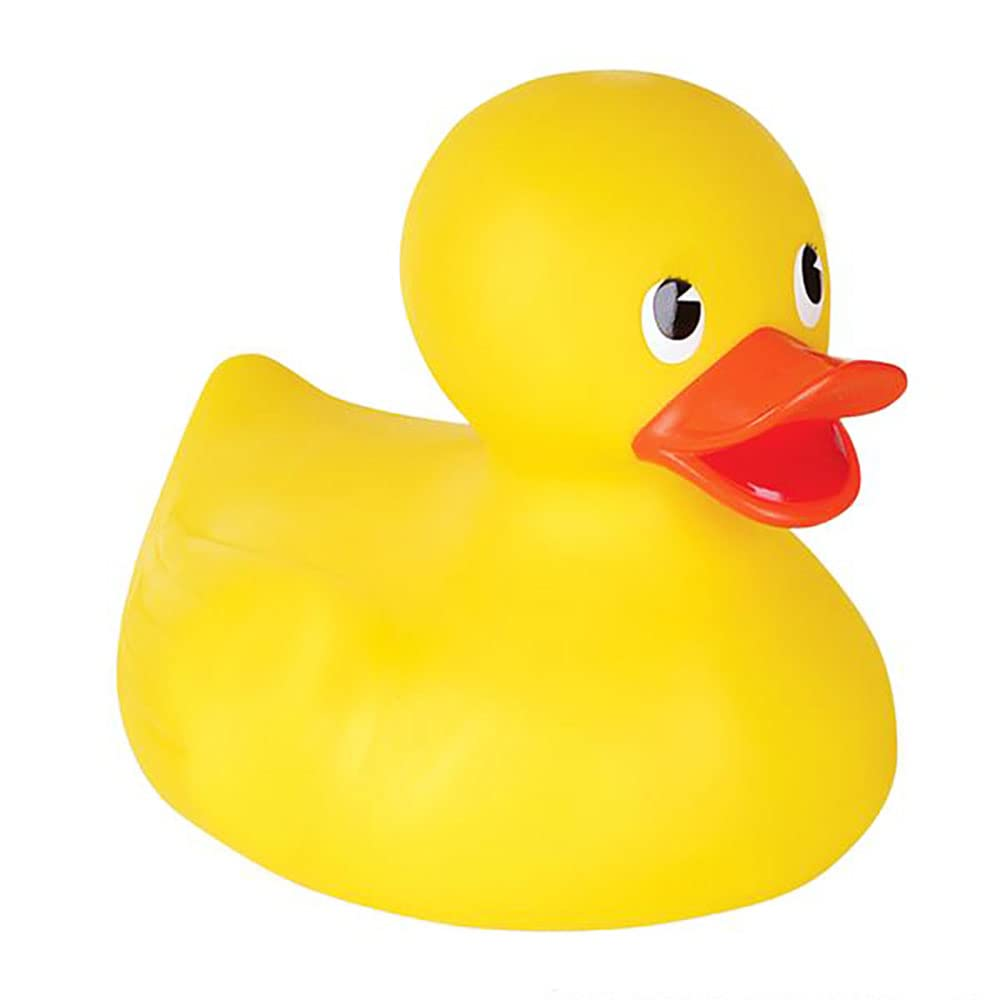
\includegraphics[scale=0.1]{document/chapters/manage_chapters/images/duck.jpeg}
    \caption{A Duck}
    \label{fig:duck}
\end{figure}
\section{Manage the Bibliography}
In \textit{"document > bibliography.bib"} you can place your bib references that will be automatically added to the document's bibliography every time you cite something \cite{https://doi.org/10.1002/job.4030130102}.

Remember that often websites offering articles also allow you download a pre-made BibTex reference that can be pasted into the .bib file.

\section{Add and use commands}
You can place your newly defined commands in \textit{"settings > commands.tex"}; this template includes the \textit{"info"} command.

\begin{info}
    This is an info
\end{info}
